\documentclass[]{article}
\usepackage[frenchb]{babel}
\usepackage[T1]{fontenc}
\usepackage{textcomp}
\usepackage[utf8]{inputenc}
\usepackage{lmodern}
\usepackage{natbib}
\usepackage{multicol}
%pour liens hypertexte
\usepackage{hyperref}
\newcommand{\mhref}[3][blue]{\href{#2}{\color{#1}{#3}}}%

\usepackage{geometry}
%\geometry{verbose,tmargin=2cm,bmargin=2cm,lmargin=2cm,rmargin=2cm}

%% The amssymb package provides various useful mathematical symbols
\usepackage{amssymb}

% Pour les tables de matières
%\usepackage{shorttoc}

%pour les tableaux
\usepackage{tabularx}
\usepackage{multirow}
\usepackage{array}
\usepackage{ctable}
\usepackage{bm}
\newcolumntype{M}[1]{>{\arraybackslash}m{#1}}

%% The amsthm package provides extended theorem environments
\usepackage{amsthm}
\usepackage{numprint}

\graphicspath{{../Figures/}}

%%Pour les algorithmes
\usepackage{algorithmic}
\usepackage{algorithm}
\usepackage{natbib}
\usepackage{bibentry}

%% Variables locales
\newcommand{\SNOT}{{SNO-Tourbières}}
\newcommand{\datasnot}{{\mhref{https://data-snot.cnrs.fr/}{data-snot}}}
\newcommand{\dataaccess}{{\mhref{https://data-snot.cnrs.fr/data-access/}{data-access}}}
\newcommand{\dataarchive}{{\mhref{https://data-snot.cnrs.fr/dataset-archive/}{dataset-archive}}}


\def\adresseMO{https://forge-osuc.cnrs-orleans.fr/projects/sie-sno-tourbiere/repository/revisions/master/entry/Documentation/Modes_operatoires/}
\def\adressedocsmetier{https://forge-osuc.cnrs-orleans.fr/projects/sie-sno-tourbiere/repository/revisions/master/entry/Documentation/Docs_metier/}

\title{Cahier des charges pour la maintenance corrective du Système d'Information du SNO-Tourbières}

\author{
	\includegraphics[scale=0.3]{logo_Tourbieres.jpg}\\[1cm]
}

\begin{document}
\maketitle
%\tableofcontents

\section{Introduction}

Ce document a pour objet de décrire les clauses techniques particulières concernant le marché de la maintenance corrective du Système d'Information du \SNOT{} (SI \SNOT).

\subsection{Objectifs}

Le \SNOT{} a décidé de confier la maintenance corrective de son Système d'Information afin d'assurer la continuité de service des applications de gestion et d'extraction des données collectées dans le \SNOT. Le \SNOT{} cherche à bénéficier des compétences d'un prestataire spécialisé et de s'assurer un service professionnel au meilleur coût.

\subsection{Services rendus}

Les prestations demandées dans le cadre de cet appel à la concurrence sont les suivantes : 

\begin{itemize}
	\item Maintenir en condition opérationnelle les applications de gestion et d'extraction des données : 
		\begin{itemize}
			\item \datasnot : application de gestion des données,
			\item \dataaccess : application de visualisation et d'extraction des données,
			\item \dataarchive : application d'extraction d'archives des jeux de données.
		\end{itemize}
	\item Assurer les mises à jours mineures de l'application \datasnot,
	\item Remonter les erreurs rencontrées dans \datasnot{} dans les Forges logicielles.\\
\end{itemize}

Ces prestations concernent donc une \textbf{maintenance corrective} du SI \SNOT. Celles-ci consistent à remettre en état de fonctionnement les logiciels et à les faire évoluer avant que des dysfonctionnements n'apparaissent.

\subsection{Identification des parties}

Le marché sera passé entre l'Observatoire des Sciences de l'Univers en région Centre (OSUC) / université d'Orléans, l'établissement porteur du \SNOT{} et le prestataire. Cette activité sera pilotée du côté du \SNOT{} par son responsable et du côté prestataire par un chef de projet nommément désigné.

\subsection{Durée}

Le marché sera conclu pour un an à compter de la date de sa notification. A l'échéance du terme, le \SNOT{} pourra décider de le reconduire d'année en année, étant entendu que la durée totale du marché ne pourra excéder trois ans. Le \SNOT{} informera par écrit le titulaire de sa décision de reconduite ou non du marché au moins trois mois avant la fin de la durée de validité du marché.

\subsection{Critères d’attribution}

Le marché sera attribué au soumissionnaire qui présentera l'offre la plus économiquement avantageuse compte-tenu des critères d’évaluations, avec leur pondération respective, listés ci-après :

\begin{itemize}
	\item Capacités techniques et financières : 20
	\item Expérience dans la réalisation de prestations similaires : 10
	\item Composition et qualité de l’équipe : 10
	\item Méthodologie proposée : 20
	\item Respect du cahier des charges : 10
	\item Coût de la prestation : 30 
\end{itemize}

La totalité de l'évaluation est effectuée sur un total de 100

\subsection{Date limite de remise des offres}

La date limite de remise des offres est fixée au ?? .\\
Les propositions devront être envoyées par courriel à : \href{mailto:contact.sno-tourbieres@cnrs-orleans.fr}{contact.sno-tourbieres@cnrs-orleans.fr}

\subsection{Modalité de règlement}

La prestation fera l'objet d’un paiement par virement administratif sur présentation d'une facture mensuelle.

\subsection{Révision du prix}

Le prix sera ferme pendant la première année d’exécution du contrat.

\section{Description de l'existant}

\subsection{Contexte}

Le Service National d'Observation des Tourbières (\SNOT) est un réseau de sites labellisés par l'Institut National des Sciences de l’Univers du CNRS (INSU-CNRS) en surfaces et interfaces continentales. Il constitue une infrastructure opérationnelle sur le long terme basée sur l'observation et la modélisation du fonctionnement des tourbières tempérées soumises aux perturbations climatiques et anthropiques.

Dans ce contexte, un Système d'Information (SI \SNOT) a été développé en interne pour gérer et diffuser les données collectées sur les 4 sites du SNO-Tourbières.

\subsection{Description générale du SI \SNOT}

Le SI \SNOT{} s'appuie sur le cycle de vie des données collectées dans le \SNOT{} : 

\begin{enumerate}
	\item La collecte des données,
	\item Le stockage et le traitement des données,
	\item L'intégration des données dans l'application \datasnot,
	\item L'extraction, la visualisation dans l'application \dataaccess,
	\item La génération d'archives accompagnées de métadonnées pour le partage des données avec d'autres SI avec \dataarchive et le module de création de métadonnées \og{}PivotMetadata\fg{}.
\end{enumerate}
	
On retrouve l'ensemble de ces étapes et l'architecture fonctionnelle dans la figure \ref{Diagramme_archifonctionnelle}.

\begin{figure}[htbp]
	\begin{center}
		%\textwidth,angle=270
		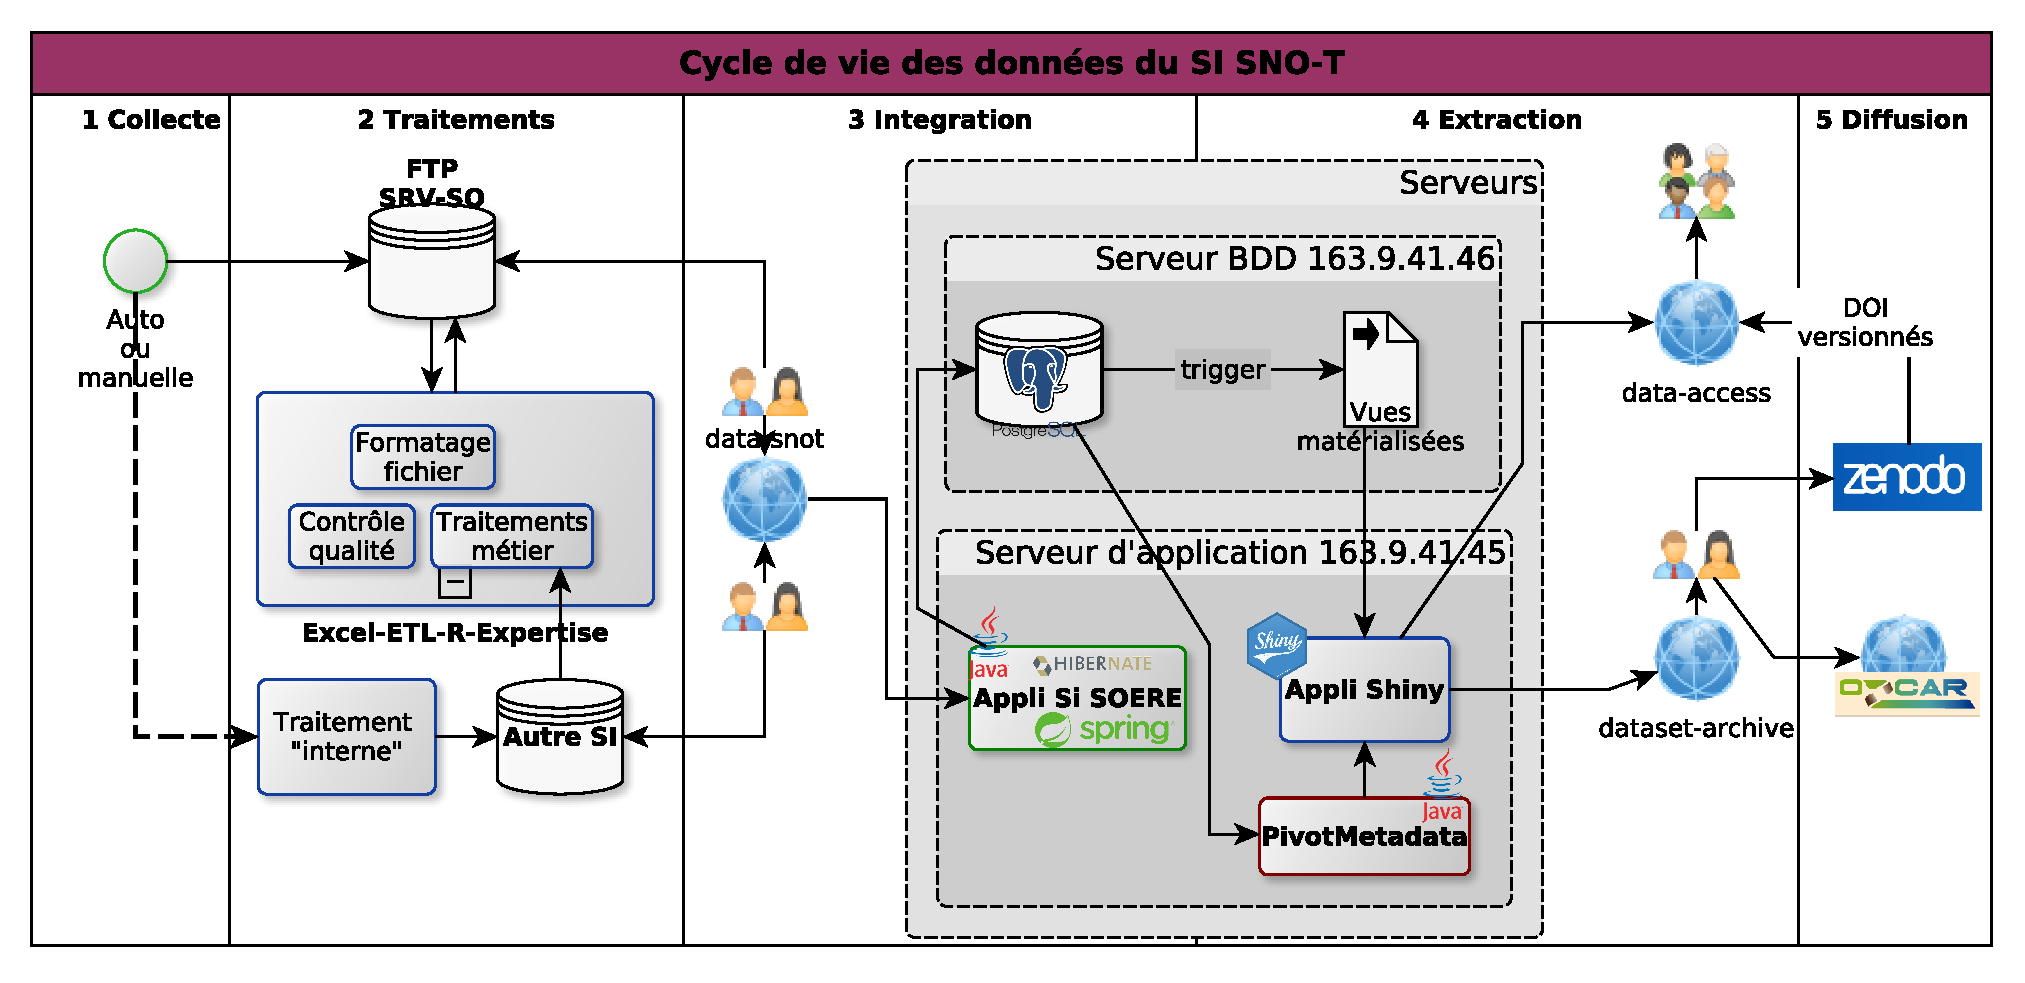
\includegraphics[width=14cm]{Diagramme_archifonctionnelle_complet.pdf}
		\caption{Architecture générale du SI \SNOT}
		\label{Diagramme_archifonctionnelle}		
	\end{center}
\end{figure}

Une documentation en ligne et une forge logicielle complète ce système d'information : 

\begin{itemize}
	\item \mhref{https://sourcesup.renater.fr/www/si-snot/5_Architecture_SI-SNOT.html}{Documentation en ligne}
	\item \mhref{https://forge-osuc.cnrs-orleans.fr/projects/sie-sno-tourbiere/}{Forge logicielle}\\
\end{itemize}

\begin{quotation}
\textbf{La maintenance corrective du SI \SNOT{} concerne uniquement les applications \datasnot, \dataaccess, \dataarchive{} et le module de création des métadonnées \og{}PivotMetadata\fg{}.}
\end{quotation}

\section{Description des prestations attendues}

\subsection{Maintenir en condition opérationnelle l'application \datasnot}

\subsubsection{Description}

L'application \datasnot{} a pour objectif d'administrer les données collectées dans le \SNOT{}. Elle s'appuie sur l'architecture et le noyau du Système d'Information des Systèmes d'Observation et d'Expérimentation au long terme pour la Recherche en Environnement (SOERE) développé par l'équipe ECO-Informatic d'InfoSol (INRA Orléans). Plus précisément, une grande partie du SI \SNOT{} est calquée sur le SI F-ORE-T en raison de la proximité des données mobilisées (flux par eddy-covariance et données méteosol notamment) :

\begin{itemize}
\item \mhref{https://git.renater.fr/authscm/jbparoisien/gitweb/?p=si-soere-kernel/documentations.git;a=blob_plain;f=techniques/Architecture_si_ecoinformatique_soere.pdf;hb=HEAD}{Architecture fonctionnelle du SI des SOERE}
\item \mhref{https://git.renater.fr/authscm/jbparoisien/gitweb/?p=si-soere-kernel/documentations.git;a=blob_plain;f=techniques/guide_du_d\%c3\%a9veloppeur/guideDeveloppeurNoyau1709.odt;hb=HEAD}{Guide de développement}
\end{itemize}

\subsubsection{Prestations attendues}

Le prestataire aura pour mission :

\begin{itemize}
	\item D'assurer les interventions curatives,
	\item De maintenir à jour l'application vis-à-vis du noyau du SI des SOERE,
	\item D'ajouter de nouveaux types de données et/ou des variables dans l'application.\\
\end{itemize}

Une documentation technique précise dans le détail le fonctionnement de l'application : 

\begin{itemize}
	\item \mhref{https://sourcesup.renater.fr/www/si-snot/5_Developper_appliSOERE.html}{Guide de développement pour \datasnot}
	\item  \mhref{https://sourcesup.renater.fr/www/si-snot/5_Deploiement_appliSOERE.html}{Guide de déploiement}
	\item  \mhref{https://sourcesup.renater.fr/www/si-snot/5_Gestion_appliSOERE.html}{Maintenance et centralisation des anomalies}
\end{itemize}

Le prestataire sera amené à interagir avec l'équipe en charge du développement du SI des SOREE.

\subsection{Maintenir en condition opérationnelle les applications \dataaccess{} et \dataarchive}

\subsubsection{Description}

Les applications \dataaccess{} et \dataarchive{} sont construites avec \mhref{https://shiny.rstudio.com/}{R-Shiny}. Elles permettent d'accéder aux données entreposées dans la base de données via l'application \datasnot.

La documentation associée à ces deux applications est dans l'onglet \og{}Procédures techniques\fg{} de la documentation à cette \mhref{https://sourcesup.renater.fr/www/si-snot/5_Administrer_shiny.html}{adresse}.

\subsubsection{Prestations attendues}

Le prestataire aura pour mission :

\begin{itemize}
	\item De gérer les incidents des serveurs,
	\item D'assurer les interventions curatives sur les deux applications,
	\item D'apporter quelques modifications dans le cas ou de nouveaux types de données seront intégrés dans \datasnot,
	\item D'apporter quelques modifications simple sur \dataarchive{} pour améliorer les archives des jeux de données en fonction du retour des utilisateurs.
\end{itemize}

\subsection{Maintenir en condition opérationnelle le service de création des métadonnées \og{}PivotMetadata\fg{}}

\subsubsection{Description}

Un service web est utilisé par l'application \dataarchive{} pour générer des archives accompagnées de métadonnées au format \og{}PIVOT\fg{}. La documentation associée à ce module (\og{}PivotMetadata\fg{}) est accessible dans la partie 
\og{}Métadonnées PIVOT (SI Theia/OZCAR)\fg{} de la documentation : 

\begin{itemize}
	\item \mhref{https://sourcesup.renater.fr/www/si-snot/5_Gestion_appliSOERE.html}{Présentation du module},
	\item \mhref{https://sourcesup.renater.fr/www/si-snot/5_Deploiement_MetadataPivot.html}{Déployer le module}.
\end{itemize}

La documentation du format \og{}PIVOT\fg{} est accessible dans la \mhref{https://theia-ozcar.gricad-pages.univ-grenoble-alpes.fr/doc-producer/producer-documentation.html}{documentation du SI Theia/OZCAR}.

\subsubsection{Prestations attendues}

Le prestataire aura pour mission :

\begin{itemize}
	\item De gérer les incidents sur le module \og{}PivotMetadata\fg{} (redémarrage du module par exemple),
	\item D'assurer les interventions curatives,
	\item D'apporter quelques modifications si le schéma du format PIVOT évolue.
\end{itemize}

\section{Contacts}

Le \SNOT{} fournira toutes les indications et instructions nécessaires à l'élaboration de la proposition.
Pour toute question, les personnes intéressées sont invitées à nous contacter par courriel : \href{mailto:contact.sno-tourbieres@cnrs-orleans.fr}{contact.sno-tourbieres@cnrs-orleans.fr}


\end{document}
